\chapter{Python 中的数据操作:numpy 与 pandas}
\dominitoc
\section{numpy 的常用操作}

numpy (Numerical Python) 是 Python 语言一个重要的扩展库,支持大量的数组与矩阵运算,此外也针对数组运算提供大量的数学函数库。numpy 通常与其他库 SciPy(Scientific Python)和 Matplotlib(绘图库)一起使用, 这种组合广泛用于模仿 MatLab 的功能。numpy 的官方手册的网址为:\href{https://numpy.org/devdocs/user/quickstart.html}{https://numpy.org/devdocs/user/quickstart.html}。

numpy 的主要功能包括:

\begin{itemize}
  \item 一个强大的 N 维数组对象 ndarray

  \item 整合 C/C++/Fortran 代码

  \item 线性代数(矩阵的各种操作)、傅里叶变换、生成随机数功能

\end{itemize}

使用 numpy 需要首先导入 numpy 包:

\begin{lstlisting}[Language=Python]
>>> import numpy as np
\end{lstlisting}

\subsection{创建数组}

用 numpy 创建数组有多种方法。首先,numpy 中的 array 方法可以直接将 Python 的 list 类型转化为 numpy 的数组类型 ndarray。例如,

一个一维数组:

\begin{lstlisting}[Language=Python]
>>> a = np.array([1, 2, 3, 4])
>>> a
array([1, 2, 3, 4])
\end{lstlisting}

一个二维数组:
\begin{lstlisting}[Language=Python]
>>> a = np.array([[1, 2], [3, 4]])
>>> a
array([[1, 2],
       [3, 4]])
\end{lstlisting}

注意,array方法中小括号中要包括一个中括号数组,而不能直接写成 np.array(1, 2, 3, 4)。

numpy 中的 zeros 方法可以创建元素值全为 0 的矩阵, ones 方法可以创建元素值全为 1 的矩阵,而 empty 方法可以创建一个元素值任意的一个空矩阵。例如:

\begin{lstlisting}[Language=Python]
>>> np.zeros((3, 4)) # 3 行 4 列的零矩阵
array([[0., 0., 0., 0.],
       [0., 0., 0., 0.],
       [0., 0., 0., 0.]])

>>> np.ones((3, 4)) # 3 行 4 列的一矩阵
array([[1., 1., 1., 1.],
       [1., 1., 1., 1.],
       [1., 1., 1., 1.]])

>>> np.empty((2, 3)) # 2 行 3 列的空矩阵
array([[0.e+000, 5.e-324, 5.e-324],
       [5.e-324, 1.e-323, 1.e-323]])
\end{lstlisting}

numpy 中的 arange 函数可以生成一个等差数列的数组,例如:

\begin{lstlisting}[Language=Python]
>>> np.arange(10) # 生成一个从 0 到 9 之间的数组,默认步长为 1
array([0, 1, 2, 3, 4, 5, 6, 7, 8, 9])

>>> np.arange(5, 10) # 生成一个从 5 到 9 之间的数组,默认步长为 1
array([5, 6, 7, 8, 9])

>>> np.arange(5, 10, 2) # 生成一个从 5 到 9 之间的数组,且步长为 2
array([5, 7, 9])
\end{lstlisting}

另外一个类似的函数为 linespace,不同的地方在于:arange 函数中第三个参数表示等差数组的步长,而 linespace 函数第三个参数表示一共生成的元素个数。若生成一系列等差的浮点数,则用 linespace 更好些。

\begin{lstlisting}[Language=Python]
>>> np.linspace(0, 2, 9 ) # 生成从 0 到 2 之间共 9 个数
array([0.  , 0.25, 0.5 , 0.75, 1.  , 1.25, 1.5 , 1.75, 2.  ])
\end{lstlisting}

\subsection{数组索引与切片}

对于一维数组,numpy 的索引切片类似 Python list 类型的索引切片,例如:

\begin{lstlisting}[Language=Python]
In [22]: a = np.arange(4, 10) # 生成一个从 4 到 9 之间的数组

In [23]: a
Out[23]: array([4, 5, 6, 7, 8, 9])

>>> a[2] # 数组 a 的第 3 个元素
6

>>> a[2:4] # 数组 a 的第 3 与第 4 个元素
array([6, 7])

>>> a[-1] # 数组 a 的最后一个元素
9

>>> a[ : : -1] # 数组 a 倒序
array([9, 8, 7, 6, 5, 4])

>>> a[3:6:2] = 4 # 将数组 a 从第 4 到 第 6 个元素间隔为 2 赋值为 4
>>> a
array([4, 5, 6, 4, 8, 4])
\end{lstlisting}

对于多维数组,numpy 数组的索引和切片用逗号分隔不同维度,例如:

\begin{lstlisting}[Language=Python]
>>> b = np.arange(12).reshape(3,4) # 创建一个 3 行 4 列的二维数组
>>> b
array([[ 0,  1,  2,  3],
       [ 4,  5,  6,  7],
       [ 8,  9, 10, 11]])

>>> b[1, 2] # 二维数组第 2 行第 3 列中的元素
6

>>> b[1:3, 2] # 二维数组第 3 列中, 第 2 行到第 3 行的元素
array([ 6, 10])

>>> b[2, :] # 第 3 行的全部元素
array([ 8,  9, 10, 11])

\end{lstlisting}

\subsection{list 数组与 array 数组互换}

Python 的自带数组类型 list 与 numpy 的 array 类型可以互换,方法是用 list() 或 np.array() 直接转换,举例:

\begin{lstlisting}[Language=Python]
In [16]: a = np.arange(4) # 一个 numpy 的 array 类型

In [17]: a
Out[17]: array([0, 1, 2, 3])

In [18]: list(a) # 将 array 类型转化成 list 类型
Out[18]: [0, 1, 2, 3]

In [19]: b = [3, 4, 5, 6]

In [20]: np.array(b) # 将 list 类型转化成 array 类型
Out[20]: array([3, 4, 5, 6])
\end{lstlisting}



\subsection{数组拼接}

Numpy 中拼接两个数组用 append 函数,举例:

\begin{lstlisting}[Language=Python]
In [27]: a = np.arange(5)

In [28]: a
Out[28]: array([0, 1, 2, 3, 4])

In [29]: b = np.arange(3)

In [30]: b
Out[30]: array([0, 1, 2])

In [31]: np.append(a, b)
Out[31]: array([0, 1, 2, 3, 4, 0, 1, 2])
\end{lstlisting}

大规模的数组拼接或者多组数组拼接,可以用 concatenate,举例:

\begin{lstlisting}[Language=Python]
In [32]: c = np.arange(4)

In [33]: c
Out[33]: array([0, 1, 2, 3])

In [35]: np.concatenate((a, b, c)) # 注意里面还有一对小括号
Out[35]: array([0, 1, 2, 3, 4, 0, 1, 2, 0, 1, 2, 3])
\end{lstlisting}



\subsection{数组运算}

numpy 可以对数组进行加减,幂运算,判断大小等,例如:

\begin{lstlisting}[Language=Python]
>>> a = np.arange(4)
>>> b = np.arange(3, 7)
>>> a
array([0, 1, 2, 3])
>>> b
array([3, 4, 5, 6])

>>> a - b # 两数组相减
array([-3, -3, -3, -3])

>>> a + b # 两数组相加
array([3, 5, 7, 9])

>>> a * 2 # 数组每个元素乘以一个数值
array([0, 2, 4, 6])

>>> a ** 2 # 数组每个元素都平方
array([0, 1, 4, 9], dtype=int32)

>>> a > 2 # 数组每个元素与一个数值比较大小
array([False, False, False,  True])

\end{lstlisting}

numpy 也支持二维数组的一些运算,包括矩阵的转置,逆矩阵,矩阵的乘积等,例如:

\begin{lstlisting}[Language=Python]
>>> a = np.array([[4.0, 5.0], [6.0, 7.0]])
>>> a
array([[4., 5.],
       [6., 7.]])
>>> b = np.array([[1.0, 2.0], [3.0, 4.0]])
>>> b
array([[1., 2.],
      [3., 4.]])

>>> a.transpose() # a 的转置矩阵
array([[4., 6.],
       [5., 7.]])

>>> np.linalg.inv(a) # a 的逆矩阵
array([[-3.5,  2.5],
       [ 3. , -2. ]])

>>> np.linalg.eig(a) # a 的特征值与特征向量
(array([-0.17890835, 11.17890835]), array([[-0.76729658, -0.57152478],
       [ 0.64129241, -0.82058481]]))

# 矩阵 a 与 b 对应元素相乘,有两种方式:使用 multiply 函数或用乘积符号 *
>>> np.multiply(a, b)
array([[ 4., 10.],
       [18., 28.]])
 >>> a * b
array([[ 4., 10.],
       [18., 28.]])

# 矩阵 a 与 b 的点积,使用 dot 函数
>>> np.dot(a, b)
array([[19., 28.],
       [27., 40.]])


\end{lstlisting}

另外,numpy 还有专门支持二维数组的类型 Matrix,可以更方便地进行一些矩阵运算,感兴趣的读者可以参见官网:

\href{https://docs.scipy.org/doc/numpy/reference/generated/numpy.matrix.html}{https://docs.scipy.org/doc/numpy/reference/generated/numpy.matrix.html}



\clearpage
\section{pandas 的常用操作}

pandas 是 Python 做统计分析时最重要的数据分析工具之一,它基于 numpy 开发,提供了许多处理大型数据集所需的函数,可以灵活高效的处理各种数据集。

pandas 一般使用两种数据类型:DataFrame 和 Series。其中 DataFrame 是二维数据,而 Series 是一维数据。可以这样简单理解:DataFrame 相当于 Excel 里面的一张表,而 Series 是表中的某一列。还有一个表示三维数据的类型 Panel,但我们经常使用的是前面两种数据类型。使用 pandas 时首先到导入 pandas 包。

\begin{lstlisting}[Language=Python]
In [3]: import pandas as pd
\end{lstlisting}

\subsection{创建、读取和存储数据}

\noindent\textbf{1. 创建数据}
 例如有下面的数据:

 \begin{table}[!ht]
 \centering
 \renewcommand{\arraystretch}{1.2}
 \begin{tabular}{|l|l|l|l|}
 \hline
 &统计学 & 高数 & 英语 \\ \hline
 张三 & 85 & 82 & 84 \\ \hline
 李四 & 68 & 63 & 90 \\ \hline
 王五 & 90 & 88 & 78 \\ \hline
 \end{tabular}
 \end{table}

我们可以使用下面的代码读取到一个 DataFrame 里面:

\begin{lstlisting}[Language=Python]
In [4]: df = pd.DataFrame({'统计学': [85, 68, 90], '高数': [82, 63, 88], '英语': [84, 90, 78]}, index=['张三', '李四', '王五'])

In [5]: df
Out[5]:
    统计学  高数  英语
张三   85  82  84
李四   68  63  90
王五   90  88  78
\end{lstlisting}

从上面可以看出,DataFrame 通过一个字典类型设置各列的标题及对应数值,通过一个 index 数组设置行标题。还有一种方式是通过 numpy 的 array 数组设置数值,然后通过 columns 数组设置列标题,通过 index 数组设置行标题\footnote{如果创建时不设置行标题或列标题,系统会自动生成从 0 到行数或列数的数组作为标题}:

\begin{lstlisting}[Language=Python]
>>> import numpy as np
>>> df = pd.DataFrame(np.array([[85, 68, 90], [82, 63, 88], [84, 90, 78]]), columns=['统计学', '高数', '英语'], index=['张三', '李四', '王五'])
\end{lstlisting}

一个 DataFrame 包括 columns(列标题),index(行标题)与 values(数值)三个部分,上述例子中的 columns, index,values 如下图所示:

\begin{figure}[!ht]
\centering
  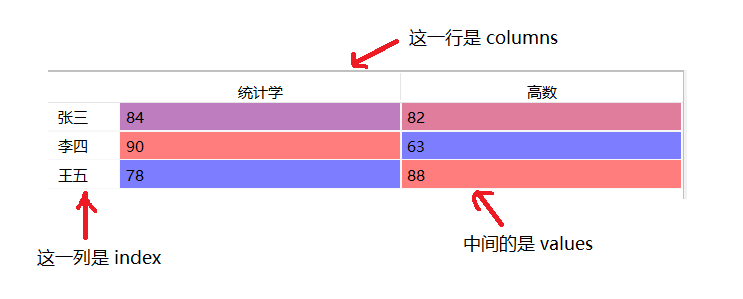
\includegraphics{figure/chapter2/pandas.png}
\end{figure}

\noindent\textbf{2. 读取数据}


大部分情况下,我们要读取 Excel 里面的数据,假设上面的例子在 excel 文件 '成绩数据.xlsx' 并放在电脑硬盘某个位置:

\begin{figure}[!ht]
\centering
  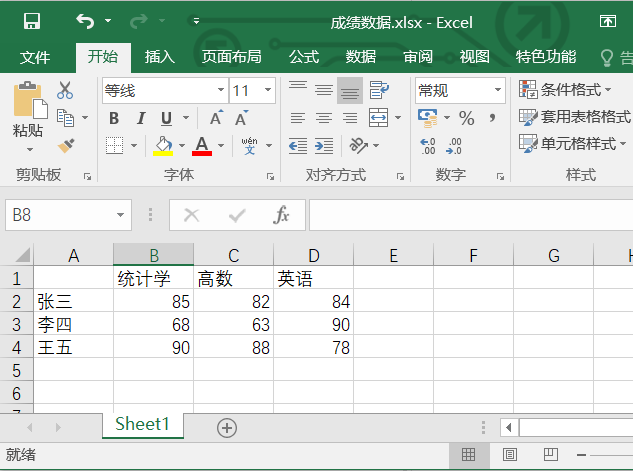
\includegraphics[scale=0.7]{figure/chapter2/pandas2.png}
\end{figure}

可以通过下面的代码读取文件:

\begin{lstlisting}[Language=Python]
>>> df = pd.read_excel(r'D:\Users\chen_\git\Statistics-book\datas\成绩数据.xlsx', index_col=0)
\end{lstlisting}

数据文件的地址位于 \path{`D:\Users\chen_\git\Statistics-book\datas\成绩数据.xlsx'},使用 read\_excel 时\textbf{在文件位置字符串前面加上字母 r},这样 Python 就能找到我们的数据文件了。index\_col=0 表示行标题位于第一列(不然 read\_excel 会把第一列内容读取到 values 里面,并默认 index 为 0, 1, 2, \dots)。read\_excel 会自动将 Excel 第一行的内容作为行标题。read\_excel 的一般语法为:

\begin{center}
\begin{tcolorbox}[title = read\_excel 函数的语法]
\textbf{read\_excel(io, sheetname=0, header=0, skiprows=None,  index\_col=None)}
\tcblower
\vspace{10pt}

\begin{tcboutputlisting}
\begin{tabular}{>{\bfseries}ll}
  io &数据文件的地址与名字,一般为字符串\\
  sheetname & 工作簿名字,默认为0,表示读取第一张工作簿\\
header &作为列名的行,默认为0,即取第一行的值为列名\\
skiprows&省略指定行数的数据,从第一行开始查起\\
index\_col&行标题所在的列\\
\end{tabular}
\end{tcboutputlisting}
\tcbuselistingtext

\end{tcolorbox}
\end{center}

\sloppy
更多的语法设置可以查看官网文档:

\href{https://pandas.pydata.org/pandas-docs/version/0.20/generated/pandas.read\_excel.html}{https://pandas.pydata.org/pandas-docs/version/0.20/generated/pandas.read\_excel.html}

还有一种常见的数据文件类型为 csv,我们只需使用 pandas 中的函数 read\_csv,它的语法与 read\_excel 基本一样。但是, read\_csv 可以读取网络数据库中的 csv 文件,例如下面的例子显示世界上所有国家与所属的大洲。

\begin{lstlisting}[Language=Python]
>>> df = pd.read_csv('https://raw.githubusercontent.com/cs109/2014_data/master/countries.csv')
>>> df
\end{lstlisting}

\begin{figure}[!ht]
\centering
  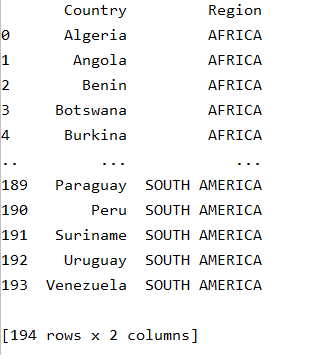
\includegraphics[scale=0.7]{figure/chapter2/pandas7.png}
\end{figure}


\noindent\textbf{3. 存储数据}

存储时使用函数 to\_excel 或 to\_csv。例如我们将 DataFrame 存储到 \path{E:\datas} 文件夹里,并命名为 marks.xlsx:

\begin{lstlisting}[Language=Python]
>>> import pandas as pd
>>> import numpy as np
>>> df = pd.DataFrame(np.array([[85, 68, 90], [82, 63, 88], [84, 90, 78]]), columns=['统计学', '高数', '英语'], index=['张三', '李四', '王五'])
>>> df.to_excel(r'E:datas\marks.xlsx')
\end{lstlisting}

在上面的代码中,若直接写成 df.to\_excel(`marks.xlsx'),则文件存储的路径为当前工作环境所在的文件夹。


\subsection{查看数据}

\noindent\textbf{1. 概览数据}

快速查看 DataFrame 各列数据的统计信息可以使用 discribe() 函数,包括各列数据的非空数值数目、均值、标准差、最大值、最小值、分位数。例如上面的例子:

\begin{lstlisting}[Language=Python]
>>> df.describe()
             统计学         高数         英语
count   3.000000   3.000000   3.000000
mean   83.666667  73.666667  85.333333
std     1.527525  14.364308   6.429101
min    82.000000  63.000000  78.000000
25%    83.000000  65.500000  83.000000
50%    84.000000  68.000000  88.000000
75%    84.500000  79.000000  89.000000
max    85.000000  90.000000  90.000000
\end{lstlisting}


info() 函数可以查看各列数据的类型:

\begin{lstlisting}[Language=Python]
>>> df.info()
<class 'pandas.core.frame.DataFrame'>
Index: 3 entries, 张三 to 王五
Data columns (total 3 columns):
统计学    3 non-null int32
高数     3 non-null int32
英语     3 non-null int32
dtypes: int32(3)
memory usage: 140.0+ bytes)
\end{lstlisting}

DataFrame 的 sample() 函数可以从数据中随机抽取样本,小括号中用数字表示抽取的样本个数。例如,下面的代码从 df 里面随机抽取 2 个样本:
\begin{lstlisting}[Language=Python]
>>> df.sample(2)
    统计学  高数  英语
王五   84  90  78
李四   82  63  88
\end{lstlisting}


另外,head() 函数可以显示 DataFrame 前五行数据,而 tail() 函数可以显示 DataFrame 最后五行数据。

\noindent\textbf{2. 查看单列、单行、单元格数据}

查看某一列数据时,最简单的方式是中括号里面输入列名的方式,例如查看英语成绩那一列数据:
\begin{lstlisting}[Language=Python]
In [17]: df['统计学']
Out[17]:
张三    85
李四    82
王五    84
Name: 统计学, dtype: int32
\end{lstlisting}

或者用一个逗点跟列名的方式,此时列名不用加引号,例如:

\begin{lstlisting}[Language=Python]
In [16]: df.统计学
Out[16]:
张三    85
李四    82
王五    84
Name: 统计学, dtype: int32
\end{lstlisting}


查看某一行数据时,最简单的方式是用中括号里面跟着行索引的方式(行数 : 行数 + 1),例如 df[0:1] 显示第一行的数据。

\begin{lstlisting}[Language=Python]
>>> df[0:1]
    统计学  高数  英语
张三   85  68  90
\end{lstlisting}

若查看某个单元格,比较方便的方式是用两个中括号,每个中括号内分别跟着行索引和列索引,例如查看李四的高数成绩:
\begin{lstlisting}[Language=Python]
>>> df[1:2]['高数']
李四    63
Name: 高数, dtype: int32
\end{lstlisting}

查看单行、单列数据,也可以用下面的 iloc 函数。

\noindent\textbf{3. 查看多列、多行数据,单行、单列数据 iloc}

查看多行、多列数据时,一般用 iloc 比较方便,而且 iloc 不仅能查看多行多列数据,也能查看单行、单列或某个单元格数据:

例如,查看行:

\begin{lstlisting}[Language=Python]
>>> df.iloc[1]          # 查看第 2 行数据
>>> df.iloc[0:2]        # 查看前 2 行数据
>>> df.iloc[[0, 2]]     # 查看第 1 行与第 3 行数据
\end{lstlisting}

查看列:

\begin{lstlisting}[Language=Python]
>>> df.iloc[:, 1]       # 查看第 2 列数据
>>> df.iloc[:, 0:2]     # 查看前 2 列数据
>>> df.iloc[:, [0, 2]]  # 查看第 1 列与第 3 列数据
\end{lstlisting}

查看一块数据:
\begin{lstlisting}[Language=Python]
>>> df.iloc[0:2, 0:2]          # 查看前 2 行,前 2 列的一块数据
>>> df.iloc[[0, 2],  [0, 2]]   # 查看第 1、第 3 行,第 1、第 3 列的一块数据
>>> df.iloc[0:2, [0, 2]]       # 查看前 3 行,第 1、第 3 列的一块数据
>>> df.iloc[[0, 2], 0:2]       # 第 1、第 3 行,前 2 列的一块数据
\end{lstlisting}

查看某个单元格:
\begin{lstlisting}[Language=Python]
>>> df.iloc[1, 1]   # 查看第 2 行,第 2 列的单元格数据
\end{lstlisting}

\noindent\textbf{4. 查看行数、列数、数据个数,行名、列名}

pandas 的 shape 方法返回数据的行数和列数的一个元组,例如:


\begin{lstlisting}[Language=Python]
In [5]: df = pd.DataFrame({'统计学': [85, 68, 90], '高数': [82, 63, 88], '英语': [84, 90, 78]}, index=['张三', '李四', '王五'])

In [6]: df
Out[6]:
    统计学  高数  英语
张三   85  68  90
李四   82  63  88
王五   84  90  78

In [7]: df.shape  # 返回 pandas 数据的行数和列数
Out[7]: (3, 3)
\end{lstlisting}


若单独返回行数,则用 shape[0],单独返回列数则用 shape[1]。

\begin{lstlisting}[Language=Python]
In [8]: df.shape[1]  # 返回 pandas 数据的列数
Out[8]: 3
\end{lstlisting}

查看 pandas 数据的所有数据元素的个数,用 size:

\begin{lstlisting}[Language=Python]
In [26]: df.size
Out[26]: 9
\end{lstlisting}


查看列名用 columns 方法, 查看所有行名用 index 方法,例如:

\begin{lstlisting}[Language=Python]
In [23]: df.columns  # 查看所有列名
Out[23]: Index(['统计学', '高数', '英语'], dtype='object')

In [24]: df.index # 查看所有行名
Out[24]: Index(['张三', '李四', '王五'], dtype='object')
\end{lstlisting}





\subsection{增加、删除、修改、查询数据}

pandas 能够像数据库一样处理数据,实现数据库的常用功能:增加数据,删除数据,修改数据,查询数据。

\vspace{3pt}
\noindent\textbf{1. 增加数据}
\vspace{3pt}

在原数据末尾增加一列时,在原数据基础上直接赋值即可,用df[`新列名'] = 新列值的形式(新列值可以是一个数,此时新列的所有值都是这个数),例如:

\begin{lstlisting}[Language=Python]
>>> import pandas as pd
>>> import numpy as np
>>> df = pd.DataFrame(np.array([[85, 68, 90], [82, 63, 88], [84, 90, 78]]), columns=['统计学', '高数', '英语'], index=['张三', '李四', '王五'])
>>> df
    统计学  高数  英语
张三   85  68  90
李四   82  63  88
王五   84  90  78

>>> df['计算机'] = [92, 69, 75] # 增加一列计算机课程的成绩
>>> df
    统计学  高数  英语  计算机
张三   85  68  90   92
李四   82  63  88   69
王五   84  90  78   75

In [75]: df['会计'] = 85 # 增加一列会计课程的成绩

In [76]: df
Out[76]:
    统计学  高数  英语  计算机  会计
张三   85  68  90   92  85
李四   82  63  88   69  85
王五   84  90  78   75  85
\end{lstlisting}
\end{lstlisting}

在原数据末尾增加一行数据时,比较简单的方式是用 loc 函数,df['新行名'] = 新行值的形式(append)

\begin{lstlisting}[Language=Python]
>>> df.loc['马六'] = [76, 82, 90, 92]
>>> df
    统计学  高数  英语  计算机
张三   85  68  90   92
李四   82  63  88   69
王五   84  90  78   75
马六   76  82  90   92
\end{lstlisting}

若要在指定位置插入列,则需要用到 insert 函数。

\begin{lstlisting}[Language=Python]
>>> df.insert(1, '运筹学', [61, 72, 84, 81]) # 在第 1 列后面插入新的一列
>>> df
    统计学  运筹学  高数  英语  计算机
张三   85   61  68  90   92
李四   82   72  63  88   69
王五   84   84  90  78   75
马六   76   81  82  90   92
\end{lstlisting}

若要在指定位置插入行,目前 pandas 还没有专门的函数,一般采用 concat 合并两个 DataFrame 的方式。例如:

\begin{lstlisting}[Language=Python]
>>> df = pd.DataFrame(np.array([[85, 68, 90], [82, 63, 88], [84, 90, 78]]), columns=['统计学', '高数', '英语'], index=['张三', '李四', '王五'])
>>> df
    统计学  高数  英语
张三   85  68  90
李四   82  63  88
王五   84  90  78

# 创建一行数据,注意 np.array 里面是双中括号
>>> df1 = pd.DataFrame(np.array([[87, 64, 71]]), columns=['统计学', '高数', '英语'], index=['陈七'])
>>> df1
    统计学  高数  英语
陈七   87  64  71

# 将这行数据通过 concat 函数插入到第一行后面,注意小括号里面有一个中括号
>>> df = pd.concat([df.iloc[: 1], df1, df.iloc[1:]])
>>> df
    统计学  高数  英语
张三   85  68  90
陈七   87  64  71
李四   82  63  88
王五   84  90  78
\end{lstlisting}

\vspace{3pt}
\noindent\textbf{2. 删除数据}
\vspace{3pt}

pandas 利用 drop 函数删除行数据或列数据。删除一行时,直接跟行标签名:

\begin{lstlisting}[Language=Python]
In [5]: df = pd.DataFrame(np.array([[85, 68, 90], [82, 63, 88], [84, 90, 78]]), columns=['统计学', '高数', '英语'], index=['张三', '李四', '王五'])

In [6]: df
Out[6]:
    统计学  高数  英语
张三   85  68  90
李四   82  63  88
王五   84  90  78

In [12]: df.drop('王五') # 删除一行
Out[12]:
    统计学  高数  英语
张三   85  68  90
李四   82  63  88
\end{lstlisting}

删除一列,除了跟列标签名外,则需要多跟一个参数 axis = 1:

\begin{lstlisting}[Language=Python]
In [14]: df.drop('英语', axis = 1)
Out[14]:
    统计学  高数
张三   85  68
李四   82  63
王五   84  90

In [15]: df
Out[15]:
    统计学  高数  英语
张三   85  68  90
李四   82  63  88
王五   84  90  78
\end{lstlisting}

从上面的代码可以看到,原始的 DataFrame并不改变,若要使得原始的 DataFrame 数据改变,需要跟一个参数 inplace = True,这个参数对于删除行或删除列的功能都一样。

\begin{lstlisting}[Language=Python]
In [18]: df.drop('英语', axis = 1, inplace = True)

In [19]: df
Out[19]:
    统计学  高数
张三   85  68
李四   82  63
王五   84  90
\end{lstlisting}

删除多行时,则需要跟所删除行的行标签名列表:
\begin{lstlisting}[Language=Python]
In [32]: df
Out[32]:
    统计学  高数  英语
张三   85  68  90
李四   82  63  88
王五   84  90  78

In [33]: df.drop(['张三', '李四'])
Out[33]:
    统计学  高数  英语
王五   84  90  78
\end{lstlisting}

删除多列时,则需要跟所删除列的列标签名列表:

\begin{lstlisting}[Language=Python]
In [36]: df
Out[36]:
    统计学  高数  英语
张三   85  68  90
李四   82  63  88
王五   84  90  78

In [37]: df.drop(['统计学', '高数'], axis = 1)
Out[37]:
    英语
张三  90
李四  88
王五  78
\end{lstlisting}

另外,也可以用 iloc 重新赋值的形式删除行列,例如:

\begin{lstlisting}[Language=Python]
In [38]: df
Out[38]:
    统计学  高数  英语
张三   85  68  90
李四   82  63  88
王五   84  90  78

In [39]: df = df.iloc[1:3, 1:3] # 只保留李四、王五的高数、英语成绩

In [40]: df
Out[40]:
    高数  英语
李四  63  88
王五  90  78
\end{lstlisting}

\vspace{3pt}
\noindent\textbf{3. 修改数据}
\vspace{3pt}

在修改 pandas 的数据时,类似查看 pandas 数据的方式,直接将 pandas 的索引位置赋值为新的值。例如,当修改某列数据时,语法为:df[`列名'] =  某个值或某个列表。


下面的代码修改统计学这一列的数值:
\begin{lstlisting}[Language=Python]
In [2]: df = pd.DataFrame(np.array([[85, 68, 90], [82, 63, 88], [84, 90, 78]]), columns=['统计学', '高数', '英语'], index=['张三', '李四', '王五'])

In [3]: df
Out[3]:
    统计学  高数  英语
张三   85  68  90
李四   82  63  88
王五   84  90  78

In [4]: df['统计学'] = 80  # 修改统计学这一列的数值为同一个值

In [5]: df
Out[5]:
    统计学  高数  英语
张三   80  68  90
李四   80  63  88
王五   80  90  78

In [6]: df['统计学'] = [95, 76, 88]  # 修改统计学这一列的数值为列表中的值

In [7]: df
Out[7]:
    统计学  高数  英语
张三   95  68  90
李四   76  63  88
王五   88  90  78
\end{lstlisting}

下面的代码修改第 2 行的数据:
\begin{lstlisting}[Language=Python]
In [9]: df.iloc[1] = 80  # 修改第 2 行的数据为同一个值

In [10]: df
Out[10]:
    统计学  高数  英语
张三   95  68  90
李四   80  80  80
王五   88  90  78

In [11]: df.iloc[1] = [95, 90, 89]  # 修改第 2 行的数据为列表中的值

In [12]: df
Out[12]:
    统计学  高数  英语
张三   95  68  90
李四   95  90  89
王五   88  90  78
\end{lstlisting}

下面的代码修改第2行第2列中的数值:

\begin{lstlisting}[Language=Python]
In [13]: df.iloc[1, 1] = 100  # 修改第2行第2列中的数值

In [14]: df
Out[14]:
    统计学   高数  英语
张三   95   68  90
李四   95  100  89
王五   88   90  78
\end{lstlisting}


\vspace{3pt}
\noindent\textbf{4. 查询数据}
\vspace{3pt}

涉及条件查询时,一般会涉及到一些比较运算符,例如:>, >=, ==, <, <=, !=(不等于)。条件查询一般只针对列数据,查询时,首先生成布尔索引,再通过指定索引进行条件查询,返回布尔值为 True 的数据。

例如,下面的代码:

\begin{lstlisting}[Language=Python]
In [15]: df = pd.DataFrame(np.array([[85, 68, 90], [82, 63, 88], [84, 90, 78]]), columns=['统计学', '高数', '英语'], index=['张三', '李四', '王五'])

In [16]: df
Out[16]:
    统计学  高数  英语
张三   85  68  90
李四   82  63  88
王五   84  90  78

In [19]: df.统计学 > 83  # 统计学成绩大于83的布尔索引
Out[19]:
张三     True
李四    False
王五     True
Name: 统计学, dtype: bool
\end{lstlisting}


\begin{lstlisting}[Language=Python]
In [20]: df[df.统计学 > 83]  # 统计学成绩大于83的数据值
Out[20]:
    统计学  高数  英语
张三   85  68  90
王五   84  90  78
\end{lstlisting}

对于多条件查询,可以用 \& 表示并:两个条件都要满足,| 表示或:两个条件满足一个即可。要注意此时每个条件外面有小括号,举例:

\begin{lstlisting}[Language=Python]
In [23]: df[(df.高数 > 65) & (df.英语 > 80)]  # 查询高数成绩大于65,英语成绩大于80的数据,注意小括号
Out[23]:
    统计学  高数  英语
张三   85  68  90
\end{lstlisting}



\subsection{排序、分组汇总}

\vspace{3pt}
\noindent\textbf{1. 排序}
\vspace{3pt}

在处理数据时,经常要对数据排序。 pandas 也提供了几种排序的方法: sort\_values,  sort\_index 等。其中,sort\_index 是对索引进行排序,而 sort\_values 是对数值进行排序,比较常用。

\begin{center}
\begin{tcolorbox}[title = sort\_values 的一般语法]
\textbf{DataFrame.sort\_values(by, axis=0, ascending=True, inplace=False,  na\_position=`last', ignore\_index=False)}
\tcblower
\vspace{10pt}

\begin{tcboutputlisting}
\begin{tabular}{>{\bfseries}ll}
  by & 需要排序的列名(axis=0)或行名(axis=1),可以有多个\\
  axis=0 & 0 表示对列排序,1 表示对行排序,默认是0\\
ascending & 升序还是降序,默认是升序排列\\
inplace & 是否替换原有数据,默认为 False 不替换 \\
na\_position&缺失值 NaN 放在排序的前面还是后面,默认是放在后面\\
ignore\_index & 如果为 True,则排序后的行号重新标号,默认是 False
\end{tabular}
\end{tcboutputlisting}
\tcbuselistingtext
\end{tcolorbox}
\end{center}

假设有下面的 pandas 数据,记录了一些学生的考试成绩:

\begin{lstlisting}[Language=Python]
In [40]: df = pd.DataFrame([['一班', '男', 85, 68, 90], ['二班', '男', 82, 63, 88], ['二班', '女',84, 90, 78], ['三班', '女',75, 68, 80],\
    ...:                    ['二班', '女',69, 55, 63], ['一班', '男', 89, 95, 93]], columns=['班级','性别','统计学','高数','英语'],\
    ...:                    index=['张三', '李四', '王五', '马六', '陈七', '魏八'])

In [41]: df
Out[41]:
    班级 性别  统计学  高数  英语
张三  一班  男   85  68  90
李四  二班  男   82  63  88
王五  二班  女   84  90  78
马六  三班  女   75  68  80
陈七  二班  女   69  55  63
魏八  一班  男   89  95  93

\end{lstlisting}


对统计学成绩升序排列:

\begin{lstlisting}[Language=Python]
In [67]: df.sort_values(by = '统计学')
Out[67]:
    班级 性别  统计学  高数  英语
陈七  二班  女   69  55  63
马六  三班  女   75  68  80
李四  二班  男   82  63  88
王五  二班  女   84  90  78
张三  一班  男   85  68  90
魏八  一班  男   89  95  93
\end{lstlisting}


对统计学与高数成绩降序排序:
\begin{lstlisting}[Language=Python]
In [69]: df.sort_values(by = ['统计学', '高数'], ascending = False)
Out[69]:
    班级 性别  统计学  高数  英语
魏八  一班  男   89  95  93
张三  一班  男   85  68  90
王五  二班  女   84  90  78
李四  二班  男   82  63  88
马六  三班  女   75  68  80
陈七  二班  女   69  55  63
\end{lstlisting}

在参数 by 中,统计学在前,高数在后,表示:先把统计学成绩降序排序,若统计学成绩有相同的,再按高数成绩降序排序。

由于排序时列标签经常被打乱,可以使用 reset\_index() 重新排列标签,原有的列标签作为新的一列,可以再跟上 drop=True 将原有的列标签去除,inplace=True 改变原始数据。

\begin{lstlisting}[Language=Python]
In [7]: df = pd.DataFrame({'统计学': [85, 68, 90], '高数': [82, 63, 88], '英语': [84, 90, 78], '姓名': ['张三', '李四', '王五']})

In [8]: df
Out[8]:
   统计学  高数  英语  姓名
0    85    82    84  张三
1    68    63    90  李四
2    90    88    78  王五

In [9]: df.sort_values(by = '统计学')  # 排序,可以看出列标也发生了变动
Out[9]:
   统计学  高数  英语  姓名
1   68      63  90  李四
0   85      82  84  张三
2   90      88  78  王五

In [10]: df.reset_index()  # 对列标签重新排列,原有的列标签作为新的一列
Out[10]:
   index  统计学  高数  英语  姓名
0      0   85  82  84  张三
1      1   68  63  90  李四
2      2   90  88  78  王五

In [13]: df.sort_values(by = '统计学').reset_index(drop = True, inplace = True) # 将原有的列标签去除,并且替换原有数据
Out[13]:
   统计学  高数  英语  姓名
0   68     63  90  李四
1   85     82  84  张三
2   90     88  78  王五
\end{lstlisting}

\vspace{3pt}
\noindent\textbf{2. 分组汇总 groupby}
\vspace{3pt}

在数据分析时,经常需要将数据分组汇总。例如,在统计学生的期末考试成绩时,可能需要根据专业或者班级来分别计算平均成绩、最高成绩等。此时,可以利用 pandas 的 groupby 函数方便地实现这些功能。



groupby 经常结合一些汇总统计量使用,例如 mean(均值),max(最大值),min(最小值),median(中位数),std(标准差),mad(平均绝对偏差),count(计数),skew(均值),quantile(分位数)。

下面的代码按性别汇总了平均成绩:

\begin{lstlisting}[Language=Python]
In [26]: df.groupby('性别').mean()  # 按性别汇总平均成绩
Out[26]:
          统计学         高数         英语
性别
女   76.000000  71.000000  73.666667
男   85.333333  75.333333  90.333333
\end{lstlisting}

若汇总列名有多个,则小括号里面放一个中括号,中括号里面跟筛选的列名,例如,下面的代码按照班级、性别汇总了平均成绩:

\begin{lstlisting}[Language=Python]
In [38]: df.groupby(['班级','性别']).mean()  按班级、性别汇总平均成绩
Out[38]:
        统计学    高数    英语
班级 性别
一班 男   87.0  81.5  91.5
三班 女   75.0  68.0  80.0
二班 女   76.5  72.5  70.5
     男   82.0  63.0  88.0
\end{lstlisting}

若要汇总多个统计量,则可以跟 agg方法,例如,下面的代码按照班级,汇总了每个班的最高、最低、平均成绩。

\begin{lstlisting}[Language=Python]
In [39]: df.groupby('班级').agg(['max', 'min', 'mean'])  # 汇总了每个班的最高、最低、平均成绩
Out[39]:
   统计学                 高数                 英语
   max  min  mean     max  min  mean     max min  mean
班级
一班  89  85  87.000000  95  68  81.500000  93  90  91.500000
三班  75  75  75.000000  68  68  68.000000  80  80  80.000000
二班  84  69  78.333333  90  55  69.333333  88  63  76.333333
\end{lstlisting}

% \vspace{3pt}
% \noindent\textbf{3. 数据透视表 pivot\_table}
% \vspace{3pt}
%
% 另外一种分组汇总的方式是使用 pivot\_table 函数,可以实现类似 excel 数据透视表的功能。
%
%
% \begin{center}
% \begin{tcolorbox}[title = pivot\_table 的语法]
% \textbf{pandas.pivot\_table(data, values=None, index=None, columns=None, aggfunc='mean', [fill\_value=None])}
% \tcblower
% \vspace{10pt}
%
% \begin{tcboutputlisting}
% \begin{tabular}{>{\bfseries}ll}
%   data &DataFrame 类型的 pandas 数据\\
% values& 可选参数,需要汇总的列,若没有则汇总所有数字列\\
% index &从原数据中选取指定的列作为数据透视表的行\\
% columns &数据透视表中保留的的列\\
% aggfunc=`mean' &可选参数,汇总的统计量,默认值是平均值\\
% fill\_value=None &可选参数,填充缺失数据的数值\\
% \end{tabular}
% \end{tcboutputlisting}
% \tcbuselistingtext
% \end{tcolorbox}
% \end{center}
%
% 举例,下面的代码对一些学生的考试成绩进行了数据透视,数据透视表的行是班级,列是性别,汇总数据为高数成绩的平均成绩:
%
% \begin{lstlisting}[Language=Python]
% In [34]: pd.pivot_table(df, index = '班级', columns = '性别', values = '高数')
% Out[34]:
% 性别     女     男
% 班级
% 一班   NaN  81.5
% 三班  68.0   NaN
% 二班  72.5  63.0
% \end{lstlisting}
%
% 因为原始数据中,一班没有女生,所以在数据透视表中,一班女生的平均成绩为缺失值 NaN。若要填充缺失值,则用 fill\_value:
%
% \begin{lstlisting}[Language=Python]
% In [35]: pd.pivot_table(df, index = '班级', columns = '性别', values = '高数', fill_value = 0)  # 将缺失值填充为零
% Out[35]:
% 性别     女     男
% 班级
% 一班   0.0  81.5
% 三班  68.0   0.0
% 二班  72.5  63.0
% \end{lstlisting}
%
% 若要汇总其他统计量,或者多个统计量,可以利用 aggfunc 定义,下面的代码汇总了平均分,最高分与最低分,
%
%
% \begin{lstlisting}[Language=Python]
% In [36]: pd.pivot_table(df, index = '班级', columns = '性别', values = '高数', aggfunc = ['mean', 'max', 'min'])
% Out[36]:
%             mean         max         min
% 性别     女     男     女     男     女     男
% 班级
% 一班   NaN  81.5   NaN  95.0   NaN  68.0
% 三班  68.0   NaN  68.0   NaN  68.0   NaN
% 二班  72.5  63.0  90.0  63.0  55.0  63.0
% \end{lstlisting}

\subsection{数据清洗}

\vspace{3pt}
\noindent\textbf{1. 数据替换 replace, fillna}
\vspace{3pt}

在进行数据处理时,经常需要对原始数据的一些异常值或错误值进行批量处理。 pandas 提供了 replace 函数方便地进行这项操作。

replace 函数第一项为原数据中的值,第二项为需要替换的值。例如,有下面的学生成绩:

\begin{lstlisting}[Language=Python]
In [19]: df = pd.DataFrame(np.array([[85, 68, 90], [82, 63, 88], [84, 90, 78]]), columns=['统计学', '高数', '英语'], index=['张三', '李四', '王五'])

In [20]: df
Out[20]:
    统计学  高数  英语
张三   85  68  90
李四   82  63  88
王五   84  90  78
\end{lstlisting}


将其中的分数 90 替换为 NaN,注意,replace方法返回了一个新的数据,原始 的 pandas 数据并没有改变

\begin{lstlisting}[Language=Python]
In [21]: df.replace(90, np.nan)
Out[21]:
    统计学    高数    英语
张三   85  68.0   NaN
李四   82  63.0  88.0
王五   84   NaN  78.0

In [22]: df  # 原始数据并没有变
Out[22]:
    统计学  高数  英语
张三   85  68  90
李四   82  63  88
王五   84  90  78
\end{lstlisting}

\textbf{若需要原始数据改变,需要跟上 inplace = True 参数},下面讲到的 fillna 方法、drop\_duplicates() 方法、dropna() 方法、 rename 方法等也可以跟这个参数使原始数据改变。

\begin{lstlisting}[Language=Python]
In [23]: df.replace(90, np.nan, inplace = True)
Out[23]:
    统计学    高数    英语
张三   85  68.0   NaN
李四   82  63.0  88.0
王五   84   NaN  78.0

In [24]: df  # 原始数据改变了
Out[24]:
     统计学 高数   英语
张三   85  68.0   NaN
李四   82  63.0  88.0
王五   84   NaN  78.0
\end{lstlisting}


pandas 还提供了 fillna 方法批量替换数据表中的确实值 NaN。例如:

\begin{lstlisting}[Language=Python]
In [7]: import numpy as np

In [8]: df = pd.DataFrame({'统计学': [85, 68, np.nan], '高数': [82, np.nan, 88], '英语': [np.nan, 90, 78]}, index=['张三', '李四', '王五'])

In [9]: df
Out[9]:
     统计学    高数    英语
张三  85.0  82.0   NaN
李四  68.0   NaN  90.0
王五   NaN  88.0  78.0

In [10]: df.fillna(80)  # 将缺失值替换为一个数值
Out[10]:
     统计学    高数    英语
张三  85.0  82.0  80.0
李四  68.0  80.0  90.0
王五  80.0  88.0  78.0

In [11]: df.fillna('missing')  # 将缺失值替换为一个字符串
Out[11]:
        统计学       高数       英语
张三       85       82  missing
李四       68  missing       90
王五  missing       88       78

In [12]: df['英语'].fillna(80)  # 对某一列的缺失值替换
Out[12]:
张三    80.0
李四    90.0
王五    78.0
Name: 英语, dtype: float64
\end{lstlisting}

pandas 还可以直接调用 isnull 方法判断数据是否为缺失值:

\begin{lstlisting}[Language=Python]
In [14]: df['英语'].isnull()
Out[14]:
张三     True
李四    False
王五    False
Name: 英语, dtype: bool
\end{lstlisting}


\vspace{3pt}
\noindent\textbf{2. 重复值处理 drop\_duplicates}
\vspace{3pt}

在数据量比较大时,经常会遇到重复数据的问题,可以使用 drop\_duplicates 将重复数据去掉。例如:

\begin{lstlisting}[Language=Python]
df = pd.DataFrame([['一班', '男', 85, 68, 90], ['一班', '男', 85, 68, 90], ['二班', '女',84, 90, 78], ['三班', '女',75, 68, 80],\
    ...:     ...:                    ['二班', '女',69, 55, 63], ['一班', '男', 89, 95, 93]], columns=['班级','性别','统计学','高数','英语'],\
    ...:     ...:                    index=['张三', '张三', '王五', '马六', '陈七', '魏八'])

In [16]: df
Out[16]:
      班级 性别  统计学  高数  英语
张三  一班  男   85  68  90
张三  一班  男   85  68  90
王五  二班  女   84  90  78
马六  三班  女   75  68  80
陈七  二班  女   69  55  63
魏八  一班  男   89  95  93
\end{lstlisting}

前两行的数据完全相同,使用 drop\_duplicates() 方法处理:

\begin{lstlisting}[Language=Python]
In [18]: df.drop_duplicates()
Out[18]:
      班级 性别  统计学  高数  英语
张三  一班  男   85  68  90
王五  二班  女   84  90  78
马六  三班  女   75  68  80
陈七  二班  女   69  55  63
魏八  一班  男   89  95  93
\end{lstlisting}

\vspace{3pt}
\noindent\textbf{3. 缺失值处理 drop\_na}
\vspace{3pt}

dropna() 方法可以将数据表中包含缺失值的行去除掉,与 drop\_duplicates() 方法相比,该方法的可调节参数更多些。它的语法如下:


\begin{center}
\begin{tcolorbox}[title = dropna 的语法]
\textbf{DataFrame.dropna(axis=0, how='any', thresh=None, inplace=False)}
\tcblower
\vspace{10pt}

\begin{tcboutputlisting}
\begin{tabular}{>{\bfseries}ll}
  axis &默认值为0,axis=0 表示删除含空值的行,\\
  &axis=1 表示删除含空值的列\\
how & 默认为 how=`any',表示若有空值,就删除,\\
&how='all',表示全部是空值才删除该行或该列\\
 thresh & 自定义数值:空值的个数,作为行或列的删除标准,默认没有\\
inplace&  默认为 False,若 inplace=True,表示处理后数据替换原数据\\
\end{tabular}
\end{tcboutputlisting}
\tcbuselistingtext
\end{tcolorbox}
\end{center}


\begin{lstlisting}[Language=Python]
In [35]: df = pd.DataFrame({'统计学': [85, 68, np.nan], '高数': [82, 75, 88], '英语': [np.nan, 90, 78]}, index=['张三', '李四', '王五'])

In [36]: df
Out[36]:
     统计学  高数    英语
张三  85.0  82   NaN
李四  68.0  75  90.0
王五   NaN  88  78.0


In [37]: df.dropna()  # 默认为删除含有空值的行,并且只要行里面有 Nan 值,就删除
Out[37]:
     统计学  高数    英语
李四  68.0  75  90.0


In [39]: df.dropna(axis = 1) # 删除含有空值的列
Out[39]:
    高数
张三  82
李四  75
王五  88

In [41]: df.dropna(how = 'all') # 全部是空值才删除
Out[41]:
     统计学  高数    英语
张三  85.0  82   NaN
李四  68.0  75  90.0
王五   NaN  88  78.0
\end{lstlisting}

\vspace{3pt}
\noindent\textbf{4. 列名重命名 rename}
\vspace{3pt}

在处理数据表时,有时候要给数据的行名后列名重命名,此时要用到 rename 方法。使用 rename 方法时,小括号中用字典形式表示替换前后的名字,替换前的名字为字典的 key,替换后的名字为字典的 value。

\begin{lstlisting}[Language=Python]
In [43]: df = pd.DataFrame({'统计学': [85, 68, 90], '高数': [82, 63, 88], '英语': [84, 90, 78]}, index=['张三', '李四', '王五'])

In [44]: df
Out[44]:
    统计学  高数  英语
张三   85  82  84
李四   68  63  90
王五   90  88  78

In [45]: df.rename(columns = {'统计学': '科目A', '高数': '科目B'})  # 更改其中两列的列名
Out[45]:
    科目A  科目B  英语
张三   85   82  84
李四   68   63  90
王五   90   88  78

In [46]: df  # 原始数据并没有发生变化
Out[46]:
    统计学  高数  英语
张三   85  82  84
李四   68  63  90
王五   90  88  78

In [47]: df.rename(columns = {'统计学': '科目A', '高数': '科目B'}, inplace = True)  # 若要原始数据变化,则附带参数 inplace = True

In [48]: df
Out[48]:
    科目A  科目B  英语
张三   85   82  84
李四   68   63  90
王五   90   88  78
\end{lstlisting}

有时候可能要更改列标签的名字,则可以通过修改 index 字典的形式使用 rename 方法:

\begin{lstlisting}[Language=Python]
In [49]: df.rename(index = {'张三': '甲', '王五': '乙'})
Out[49]:
    科目A  科目B  英语
甲    85   82  84
李四   68   63  90
乙    90   88  78
\end{lstlisting}



\subsection{时间序列数据的处理}

\vspace{3pt}
\noindent\textbf{1. to\_datetime 与 dt.strftime}
\vspace{3pt}

实际工作中,经常会遇到大量的时间序列数据。这些时间序列的原始数据一般为文本格式,我们需要将它转化为时间日期格式。 pandas 提供了 to\_datetime 方法将其他格式转化为 python 标准的日期时间格式。例如:

\begin{lstlisting}[Language=Python]
In [19]: pd.to_datetime('20200514')
Out[19]: Timestamp('2020-05-14 00:00:00')

In [20]: pd.to_datetime('2020/05/14')
Out[20]: Timestamp('2020-05-14 00:00:00')

In [21]: pd.to_datetime('2020-05-14')
Out[21]: Timestamp('2020-05-14 00:00:00')
\end{lstlisting}

在上面的代码中可以看出,to\_datetime 方法将不同类型的时间数据都转化为:年-月-日 时:分:秒格式。还可以通过 dt.strftime 方法将 pandas 某一列时间数据转化为不同格式的字符串,例如:

\begin{lstlisting}[Language=Python]
In [58]: df = pd.DataFrame({'入校时间': ['2016-09-15', '2017-03-23', '2018-09-05'], '统计学': [85, 68, 90], '高数': [82, 63, 88], '英语': [84, 90, 78], '姓名': ['张三', '李四', '王五']})

In [59]: df
Out[59]:
         入校时间  统计学  高数  英语  姓名
0  2016-09-15   85  82  84  张三
1  2017-03-23   68  63  90  李四
2  2018-09-05   90  88  78  王五

In [60]: df.iloc[0, 0]  # 原始数据中的时间为字符串
Out[60]: '2016-09-15'

In [61]: df['入校时间'] = pd.to_datetime(df['入校时间']) # 将原始数据中的时间转化为 python 的日期格式

In [62]: df.iloc[0, 0]
Out[62]: Timestamp('2016-09-15 00:00:00')

In [63]: df['入校时间'].dt.strftime('%m-%d-%y')  # 将日期格式转化为自定义格式的字符串
Out[63]:
0    09-15-16
1    03-23-17
2    09-05-18
Name: 入校时间, dtype: object

In [64]: df['入校时间'].dt.strftime('%B-%d-%y')  # 将日期格式转化为自定义格式的字符串,小写 Y 年份显示两位
Out[64]:
0    September-15-16
1        March-23-17
2    September-05-18
Name: 入校时间, dtype: object

In [65]: df['入校时间'].dt.strftime('%B-%d-%Y')  # 将日期格式转化为自定义格式的字符串,大写 Y 则年份显示四位
Out[65]:
0    September-15-2016
1        March-23-2017
2    September-05-2018
Name: 入校时间, dtype: object

In [66]: df['入校时间'].dt.strftime('%Y-%W')  # 将日期格式转化为自定义格式的字符串,大写 W 显示的为该年第几周
Out[66]:
0    2016-37
1    2017-12
2    2018-36
Name: 入校时间, dtype: object

In [76]: df['入校时间'].dt.strftime('%Y-%m-%w')  # 将日期格式转化为自定义格式的字符串,小写 w 显示的为该月第几周
Out[76]:
0    2016-09-4
1    2017-03-4
2    2018-09-3
Name: 入校时间, dtype: object
\end{lstlisting}

\vspace{3pt}
\noindent\textbf{2. resample 聚合时间数据}
\vspace{3pt}

对于很多时间序列数据,有时候经常需要对它们按一定周期合并,可以用 pandas 提供的 resample 方法。resample 方法中的小括号中用不同参数表示聚合的频率。举例:

\begin{lstlisting}[Language=Python]
In [83]: import numpy as np

In [88]: index = pd.date_range('24/12/2019', periods=10, freq='D')  # 生成一个时间序列,频率为天,周期数为 10

In [89]: index
Out[89]:
DatetimeIndex(['2019-12-24', '2019-12-25', '2019-12-26', '2019-12-27',
               '2019-12-28', '2019-12-29', '2019-12-30', '2019-12-31',
               '2020-01-01', '2020-01-02'],
              dtype='datetime64[ns]', freq='D')

In [90]: df = pd.DataFrame(np.arange(10),index = index)  # 创建一个包含时间序列的 DataFrame 数据表

In [91]: df
Out[91]:
            0
2019-12-24  0
2019-12-25  1
2019-12-26  2
2019-12-27  3
2019-12-28  4
2019-12-29  5
2019-12-30  6
2019-12-31  7
2020-01-01  8
2020-01-02  9

In [92]: df.resample('M').sum()  # 用 resample 方法按月('M')对数据聚合
Out[92]:
             0
2019-12-31  28
2020-01-31  17

In [95]:

In [95]: df.resample('3D').sum()  # 用 resample 方法每 3 天('3D')对数据聚合
Out[95]:
             0
2019-12-24   3
2019-12-27  12
2019-12-30  21
2020-01-02   9

In [96]: df.resample('w').sum()  # 用 resample 方法每周('w')对数据聚合
Out[96]:
             0
2019-12-29  15
2020-01-05  30
\end{lstlisting}

resample 定义聚合频率的参数中, `T' 表示分钟,`H' 表示小时,这些参数用大小写均可,作用相同(这一点与 dt.strftime 方法中的时间日期格式不一样)。

\subsection{数据转化为数组或列表,数据旋转}

使用 pandas 中的 values 方法可以将 pandas 数据转化为 numpy 的数组形式。例如,对于前面的 pandas 数据例子:

\begin{lstlisting}[Language=Python]
In [12]: df.values
Out[12]:
array([[85, 68, 90],
       [82, 63, 88],
       [84, 90, 78]])
\end{lstlisting}

若只要某一列的数据转化为 numpy 数据类型,则通过查看该列数据的方式,后面跟上 values,例如,将统计学成绩转化为 numpy 数组:

\begin{lstlisting}[Language=Python]
In [18]: df['统计学'].values  # 或 df.统计学.values
Out[18]: array([85, 82, 84])
\end{lstlisting}

也可以对某列数据,使用 tolist() 方法,将该列数据转化为 python 本身的列表类型 list:

\begin{lstlisting}[Language=Python]
In [51]: df['英语'].tolist()
Out[51]: [84, 90, 78]
\end{lstlisting}


pandas 还提供了一个数据旋转功能 pivot,可以将数据表中的某几列数据重新组合成一个新的数据表 DataFrame。 下面的例子中,将班级作为行标签,姓名作为列标签,高数成绩为数值,组成了一个新的数据表。

\begin{lstlisting}[Language=Python]
In [17]: df = pd.DataFrame({'班级': ['一班', '二班', '一班'], '姓名': ['张三', '李四', '王五'], '统计学': [85, 68, 90], '高数': [82, 63, 88], '英语': [84, 90, 78]})

In [18]: df
Out[18]:
   班级  姓名  统计学  高数  英语
0  一班  张三   85  82  84
1  二班  李四   68  63  90
2  一班  王五   90  88  78

In [19]: df.pivot(index = '班级', columns = '姓名', values = '高数')  # 将班级作为行标签,姓名作为列标签,高数成绩为数值
Out[19]:
姓名    张三    李四    王五
班级
一班    82.0   NaN    88.0
二班     NaN   63.0   NaN
\end{lstlisting}

\subsection{数据合并}

pandas 中比较常用的两个合并数据的方法是 concat 与 merge。 当两个 pandas 数据表具有完全相同的列名时(\textbf{相同字段的首尾相接}),一般用 concat 合并,其他情况下多用 merge 合并。

\vspace{3pt}
\noindent\textbf{1. 首尾合并 concate }
\vspace{3pt}

假如有下面两个 pandas 数据:

\begin{lstlisting}[Language=Python]
In [43]: df1 = pd.DataFrame({'统计学': [85, 68, 90], '高数': [82, 63, 88], '英语': [84, 90, 78]}, index=['张三', '李四', '王五'])
In [44]: df1
Out[44]:
   姓名  统计学  高数  英语
0  张三   85  82  84
1  李四   68  63  90
2  王五   90  88  78

In [45]: df2 = pd.DataFrame({'姓名': ['马六', '陈八'], '统计学': [83, 59], '高数': [92, 70], '英语': [94, 78]})

In [46]: df2
Out[46]:
   姓名  统计学  高数  英语
0  马六   83  92  94
1  陈八   59  70  78
\end{lstlisting}

两张表具有完全相同的行名,只是将一张数据表添加到另一个数据表后面,用 concat 合并的代码如下:

\begin{lstlisting}[Language=Python]
In [48]: pd.concat([df1, df2])  #  注意中括号不等丢
Out[48]:
   姓名  统计学  高数  英语
0  张三   85  82  84
1  李四   68  63  90
2  王五   90  88  78
0  马六   83  92  94
1  陈八   59  70  78
\end{lstlisting}

若要合并后的 index 重新命名,可以加参数 ignore\_index=True:

\begin{lstlisting}[Language=Python]
In [49]: pd.concat([df1, df2], ignore_index=True)
Out[49]:
   姓名  统计学  高数  英语
0  张三   85  82  84
1  李四   68  63  90
2  王五   90  88  78
3  马六   83  92  94
4  陈八   59  70  78
\end{lstlisting}

可以看出,加了 ignore\_index=True 之后,合并后数据的 index 重新从小到大命名。假如有下面的数据:

\begin{lstlisting}[Language=Python]
In [52]: df3 = pd.DataFrame({'姓名': ['张三', '李四', '王五'], '会计': [75, 78, 80], '管理学': [94, 96, 88]})

In [53]: df3
Out[53]:
   姓名  会计  管理学
0  张三  75   94
1  李四  78   96
2  王五  80   88
\end{lstlisting}

df1 与 df3 的姓名相同,但列名不完全相同。我们想把 df3 的列添加到 df1 中,此时就要使用 merge 方法了。

\vspace{3pt}
\noindent\textbf{2. 匹配合并 merge }
\vspace{3pt}

pandas 利用 merge 方法将两个 DataFrame 类型合并。merge 方法的一般语法如下:


\begin{center}
\begin{tcolorbox}[title = merge 的语法]
\textbf{DataFrame.merge(right, how=`inner', on=None)}
\tcblower
\vspace{10pt}

\begin{tcboutputlisting}
\begin{tabular}{>{\bfseries}ll}
  right &需要合并的另一个 pandas 数据\\
how & 默认为 `inner',表示内连接,取两个数据表中所匹配字段的交集进行合并\\
 & `outer',表示外连接,取两个数据表中所匹配字段的并集进行合并\\
&  `left',表示左连接,取左边数据表中的所匹配字段进行合并\\
 & `right',表示右连接,取右边数据表中的所匹配字段进行合并\\
on &匹配的字段(列),可以是一个或多个\\
\end{tabular}
\end{tcboutputlisting}
\tcbuselistingtext
\end{tcolorbox}
\end{center}

因此,对于 df1 与 df3,用 merge 合并时,匹配的字段(列名)为 `姓名':

\begin{lstlisting}[Language=Python]
In [66]: df1.merge(df3, on = '姓名')
Out[66]:
   姓名  统计学  高数  英语  会计  管理学
0  张三   85     82    84     75    94
1  李四   68     63    90     78    96
2  王五   90     88    78     80    88
\end{lstlisting}

merge 也能实现首尾相接的合并,例如,合并 df1 与 df2:

\begin{lstlisting}[Language=Python]
In [65]: df1.merge(df2, on = ['姓名', '统计学', '高数', '英语'], how = 'outer')
Out[65]:
   姓名  统计学  高数  英语
0  张三    85     82  84
1  李四    68     63  90
2  王五    90     88  78
3  马六    83     92  94
4  陈八    59     70  78
\end{lstlisting}

在上面的代码中,匹配的字段为所有的列,连接方式为外连接,实现结果与 concat 相同。若连接方式为其他类型,显示效果如下:

\begin{lstlisting}[Language=Python]
In [67]: df1.merge(df2, on = ['姓名', '统计学', '高数', '英语'], how = 'inner')  # 内连接时两个数据表匹配字段的交集为空
Out[67]:
Empty DataFrame
Columns: [姓名, 统计学, 高数, 英语]
Index: []

In [68]: df1.merge(df2, on = ['姓名', '统计学', '高数', '英语'], how = 'left')  # 左连接时保留左数据表的所有匹配字段
Out[68]:
   姓名  统计学  高数  英语
0  张三   85  82  84
1  李四   68  63  90
2  王五   90  88  78

In [69]: df1.merge(df2, on = ['姓名', '统计学', '高数', '英语'], how = 'right')  # 右连接时保留右数据表的所有匹配字段
Out[69]:
   姓名  统计学  高数  英语
0  马六   83  92  94
1  陈八   59  70  78
\end{lstlisting}

可以看出,\textbf{使用 merge 合并数据表时, on 中匹配的字段一般是两个数据表中完全相同的列}。 在合并数据表时,若某些字段没有对应数据,panda 会自动用 NaN 替代。下面的例子与图片展示了不同连接方式的效果。

\begin{lstlisting}[Language=Python]
In [2]: df1 = pd.DataFrame({'班级': ['一班', '二班', '一班'], '姓名': ['张三', '李四', '王五'], '性别': ['男', '男', '女'], '籍贯': ['北京', '上海', '重庆']})

In [3]: df2 = pd.DataFrame({ '姓名': ['张三', '陈八'], '统计学': [85, 59]})

In [4]: df1
Out[4]:
   班级  姓名 性别  籍贯
0  一班  张三  男  北京
1  二班  李四  男  上海
2  一班  王五  女  重庆

In [5]: df2
Out[5]:
   姓名  统计学
0  张三   85
1  陈八   59

In [6]: df1.merge(df2, on = '姓名')
Out[6]:
   班级  姓名 性别  籍贯  统计学
0  一班  张三  男  北京   85

In [7]: df1.merge(df2, on = '姓名', how = 'outer') # 某些字段没有对应数据,则显示为 NaN
Out[7]:
    班级  姓名   性别   籍贯   统计学
0   一班  张三    男   北京  85.0
1   二班  李四    男   上海   NaN
2   一班  王五    女   重庆   NaN
3    NaN  陈八   NaN   NaN  59.0

In [8]: df1.merge(df2, on = '姓名', how = 'left')
Out[8]:
   班级  姓名 性别  籍贯   统计学
0  一班  张三  男  北京  85.0
1  二班  李四  男  上海   NaN
2  一班  王五  女  重庆   NaN

In [9]: df1.merge(df2, on = '姓名', how = 'right')
Out[9]:
    班级  姓名   性别   籍贯  统计学
0   一班  张三    男   北京   85
1    NaN  陈八    NaN  NaN   59
\end{lstlisting}


\begin{figure}[!ht]
\centering
  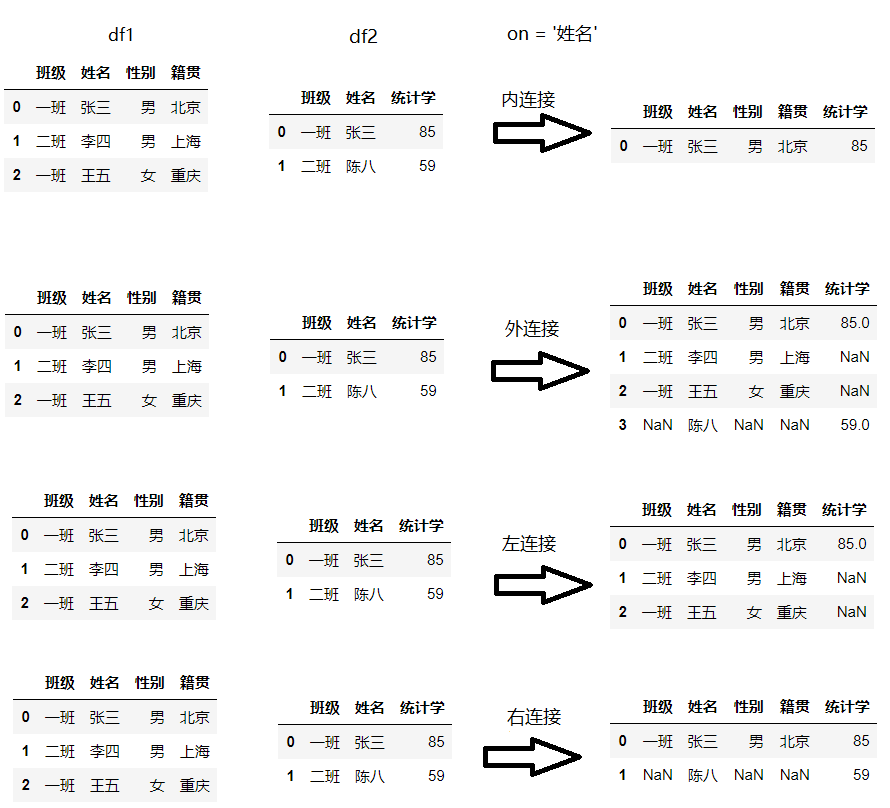
\includegraphics[scale=0.75]{figure/merge.png}
\end{figure}

\subsection{调用函数 apply、applymap}


pandas 可以直接调用函数处理数据,函数既可以是一些宏包中的函数,也可以是自定义函数,这就要用到 apply 或 applymap 方法。

\begin{center}
\begin{tcolorbox}[title = apply 的一般语法]
\textbf{DataFrame.apply(func, axis=0)}
\tcblower
\vspace{10pt}

\begin{tcboutputlisting}
\begin{tabular}{>{\bfseries}ll}
  func & pandas 调用的函数\\
axis & 取值为 0 表示调用函数作用于每一列,\\
&取值为 1 表示调用函数作用于每一行,默认值为 0\\
\end{tabular}
\end{tcboutputlisting}
\tcbuselistingtext
\end{tcolorbox}
\end{center}


对上面例子中的每个数据开根号:

\begin{lstlisting}[Language=Python]
In [50]: df.apply(np.sqrt)
Out[50]:
         统计学        高数        英语
张三  9.219544  8.246211  9.486833
李四  9.055385  7.937254  9.380832
王五  9.165151  9.486833  8.831761
\end{lstlisting}

假如我们使用 lambda 函数定义了一个最大值减去最小值的函数,并使用 apply 调用:

\begin{lstlisting}[Language=Python]
In [59]: df.apply(lambda x : max(x) - min(x))  # 对每一列调用函数
Out[59]:
统计学     3
高数     27
英语     12
dtype: int64

In [60]: df.apply(lambda x : max(x) - min(x), axis = 1)  # 对每一行调用函数
Out[60]:
张三    22
李四    25
王五    12
dtype: int64
\end{lstlisting}

需要注意的是,\textbf{对整个 DataFrame 类型使用 apply 方法时,传递的参数是一整列或一整行的所有元素}。当调用的函数的输入参数仅为单个元素时,则不能对直接使用 apply 方法,只能对某一行或某一列使用函数。

例如,下面定义一个成绩替换函数,将分数替换为``优良中差”:

\begin{lstlisting}[Language=Python]
def replace_score(x):
    if x >= 90:
        return '优'
    elif x >= 80:
        return '良'
    elif x >= 60:
        return '中'
    else:
        return '差'
\end{lstlisting}

由于上面的函数的输入参数为单个元素,所以我们只能对某一行或某一列使用 apply:

\begin{lstlisting}[Language=Python]
In [55]: df.统计学.apply(replace_score)  # 对统计学这一列使用 apply
Out[55]:
张三    良好
李四    良好
王五    良好
Name: 统计学, dtype: object

In [61]: df.iloc[0].apply(replace_score)  # 对张三这一行使用 apply
Out[61]:
统计学    良好
高数     中等
英语     优秀
Name: 张三, dtype: object
\end{lstlisting}

在上面的代码中,若对 df 直接使用 apply 方法调用函数:df.apply(replace\_score),则会报错。

另外一个直接作用于 pandas 数据所有元素的方法为 applymap。例如,上面的自定义函数 replace\_score 可以使用 applymap 调用,对 df 的每一个数据进行替换:

\begin{lstlisting}[Language=Python]
In [62]: df.applymap(replace_score)
Out[62]:
   统计学  高数  英语
张三  良好  中等  优秀
李四  良好  中等  良好
王五  良好  优秀  中等
\end{lstlisting}
